% Initial research manuscript, NOT peer reviewed, EXPLORATORY. NOT COMPILED: no LaTeX toolchain was available
% (kpsewhich/pdflatex absent). If ieeeaccess.cls is installed, replace the documentclass line with
% \documentclass{ieeeaccess} and adapt the title block; the content files are class-independent.
\documentclass[journal]{IEEEtran}
\usepackage{cite}
\usepackage{amsmath,amssymb}
\usepackage{graphicx}
\usepackage{url}
\usepackage{xcolor}
\usepackage{array}
\usepackage{hyperref}
\def\BibTeX{{\rm B\kern-.05em{\sc i\kern-.025em b}\kern-.08em T\kern-.1667em\lower.7ex\hbox{E}\kern-.125em X}}
\newcommand{\NDO}{\texttt{NO\_DIVERGENCE\_OBSERVED}}
\newcommand{\DIV}{\texttt{DIVERGENT\_OBSERVABLE}}
\newcommand{\INS}{\texttt{INSUFFICIENT}}
\newcommand{\NE}{\textbf{NOT EVALUATED}}
% Diagrams are Graphviz .dot sources. If a rendered PDF exists next to the source it is included,
% otherwise a placeholder box naming the unrendered source is printed.
\newcommand{\dotfig}[3]{\begin{figure}[t]\centering
 \IfFileExists{figures/#1.pdf}{\includegraphics[width=\columnwidth]{figures/#1.pdf}}%
 {\fbox{\parbox{0.9\columnwidth}{\footnotesize UNRENDERED diagram. Source: \path{figures/#1.dot} (render with \texttt{dot -Tpdf}).}}}
 \caption{#2 (diagram source \path{figures/#1.dot}, not rendered in this submission.)}\label{#3}\end{figure}}
\begin{document}
\title{Evidence-Sufficient Differential Behavioural Analysis for Software Evolution: A Witness-Based Approach}
\author{\IEEEauthorblockN{Anonymous author(s)}\IEEEauthorblockA{Initial research manuscript, not peer reviewed, exploratory}}
\maketitle
\begin{center}\fbox{\parbox{0.92\columnwidth}{\footnotesize\textbf{Initial research manuscript, not peer reviewed, exploratory.} All empirical results are on non-pristine development data and are descriptive only. No confirmatory evaluation exists.}}\end{center}
\begin{abstract}
When a program changes, a differential check that finds no difference is easily read as reassurance, although it only reports what the chosen inputs exercised. We describe V7-B, a prototype that compares two versions of a Python function by executing both, and that emits exactly one of three verdicts: \DIV{} backed by a replayable witness, \INS{} with a coded reason, or \NDO{} with a recorded sufficiency level (S1 or S2) that states how much of the changed code was exercised. No equivalence verdict exists. Evidence is stored as content-addressed, hash-chained records so that a verdict can be traced to the runs behind it. We evaluate the prototype only exploratorily on 321 development pairs, all of which are exposed or non-pristine (QuixBugs, BugsInPy function units, synthetic mutants). On these data V7-B detects 0.708 of the 106 pairs with a divergent label, against 0.774 for plain same-input differential execution (B1); adding the same repetition counts to B1 (B1+rep) changes the verdict on only 2 of 321 pairs, and the sufficiency level does not visibly separate generator labels. V7-B abstains on 0.360 of 258 primary pairs, mostly because of unimplemented engine features rather than a meaningful sufficiency judgement. Power on the observed design is too low for a confirmatory claim, the real-pair feasibility gate K1 is not met, and no published tool was compared. We therefore present V7-B as a design and feasibility report with negative and null findings, not as a validation.

\end{abstract}
\begin{IEEEkeywords}
differential testing, behavioural regression, software evolution, witness, evidence sufficiency, abstention, reproducibility, exploratory evaluation

\end{IEEEkeywords}
\section{Introduction}\label{sec:intro}
Checking a code change by running the old and the new version on the same inputs is a long-standing practice~\cite{evans2007,palikareva2016,jin2010automated}, and recent work uses large language models to generate the inputs~\cite{etemadi2024mokav,pradel2025testora,hu2026difftestgen,liu2025evaluating}. A difference found this way is actionable. The absence of a difference is not: it holds only for the executions that were observed, and a change that was never reached by any input produces the same silence as a change that was exercised and found harmless.

This paper describes V7-B, a research prototype built around one design rule: a ``no difference'' outcome must carry a record of how much of the change was exercised, and must be withheld when that record is inadequate or when nondeterminism, resource limits or engine gaps make the comparison unreliable. The prototype is implemented for Python functions and evaluated only on development data. We state the scope early because the evidence is limited: all 321 evaluation pairs are exposed or non-pristine, the feasibility gate for real projects is not met, and the central design element (the sufficiency level) shows no measured benefit in these data (Section~\ref{sec:results}).

The contribution is therefore an explicit design, an implementation status report, and an honest negative and null result set, offered so that a confirmatory study can be designed on firmer ground. Section~\ref{sec:rqs} lists the claims we do and do not make.

\section{Motivation}\label{sec:motivation}
Consider a reviewer who runs a differential check on a refactoring and sees ``no difference''. Three situations produce the same output: the changed lines ran and behaved identically; the changed lines never ran; or the comparison was unreliable (flaky output, a timeout on one side, a missing entry point). A tool that reports all three as ``pass'' invites false assurance. Impact-analysis authors have long noted that their results hold only for observed executions~\cite{law2003,orso2003}, and invariant-based work notes that accuracy depends on test quality~\cite{ernst2001}. Change coverage is measured in practice~\cite{hilton2018a}, but as a property of a test suite rather than as a condition on the reported outcome.

The question that motivates V7-B is narrow and empirical: if the verdict is made conditional on a recorded sufficiency level and on reproducibility checks, does the resulting ``no difference'' carry measurably less false assurance than a same-budget baseline that has repetition but no sufficiency gate? We could not answer that question here (Section~\ref{sec:results}); we describe the mechanism and what the development data do and do not show.

\section{Related Work}\label{sec:related}
This review is thematic and limited: it was produced by a single reviewer, most statements rest on abstracts or metadata, and ``we found none'' statements are not proofs of absence. Table~\ref{tab:capability} compares capabilities only where the source text supports a label.

\textbf{Cross-version differential execution.} Differential testing for change detection predates our setting~\cite{evans2007}; behavioural regression testing~\cite{jin2010automated}, DiffGen-style unit-test generation~\cite{taneja2008diffgen}, REST differential regression testing~\cite{godefroid2020differential}, and shadow symbolic execution~\cite{palikareva2016} execute versions side by side. Recent LLM-based tools target difference-exposing tests: Mokav~\cite{etemadi2024mokav}, Testora~\cite{pradel2025testora}, DiffTestGen~\cite{hu2026difftestgen}, the regression-test-generation study of Liu et al.~\cite{liu2025evaluating} (which we refer to as Cleverest) and DiffSpec~\cite{rao2024diffspec}. These are the closest competitors on discovering differences; none was run in our study.

\textbf{Change coverage and impact.} Whether tests touch the change is studied as coverage~\cite{hilton2018a}; DiffTestGen uses a union coverage of modified code as generation feedback~\cite{hu2026difftestgen}; dynamic impact analysis states its limits relative to observed runs~\cite{law2003,orso2003}. From the abstracts read, none makes change coverage a precondition of the reported verdict (a weak, abstract-level observation). Coverage as a proxy for evidence strength is itself contested~\cite{inozemtseva2014coverage,just2014mut}, which is a threat to our sufficiency definition.

\textbf{Sound equivalence and inconclusive outcomes.} Regression verification~\cite{godlin2009,felsing2014} and DiffKemp~\cite{malik2021} target equivalence statically; DiffKemp already has an undetermined outcome, whose reasons concern analysability rather than observation sufficiency. Abstention is established in machine learning~\cite{chow1970on,geifman2017,hendrickx2024machine} and applied to code models~\cite{spiess2025calibration}, but on model confidence rather than observational evidence.

\textbf{Witnesses.} Verification witnesses are exchangeable, independently validated artefacts in software verification~\cite{beyer2022verification,beyer2015witness,beyer2016correctness}. In cross-version testing, witnesses are concrete difference-exposing inputs~\cite{palikareva2016,etemadi2024mokav}.

\textbf{Flakiness and reproducibility.} Flaky tests are heavily studied~\cite{luo2014an,lam2019idflakies,parry2021a}, and LLM output nondeterminism threatens reproducibility~\cite{ouyang2025an}. Re-running to filter flaky differences is standard practice, so repetition alone is not a contribution.

\textbf{Novelty assessment.} Each primitive has prior art. A replayable witness carrying observation context, a recorded sufficiency field gating the verdict, an observation-grounded inconclusive outcome, and flakiness evidence inside a cross-version verdict are each classified in our assessment as at most partially novel, and we use no ``first'' or ``state of the art'' wording. The defensible contribution is the integration under one record contract. Empirical benefit of that integration is unsupported by this work.

\begin{table*}[t]
\centering\scriptsize
\caption{Capability comparison from the project's related-work review (\path{research/literature/RELATED_WORK_COMPARISON.md}). Labels: S = Supported, P = Partially supported, N = Not supported (full-text source states it), NE = Not evaluated (source silent at the access level read; silence is not evidence of absence), U = Unknown (access too low), NA = Not applicable. Capabilities: (A) executes both versions; (B) re-checkable witness; (C) sufficiency record; (D) evidence-grounded inconclusive outcome; (E) nondeterminism handling; (F) real-change evaluation. Cells reflect the cited text only, mostly abstracts; the last row is this work's own implementation, not a run of any compared tool.}
\label{tab:capability}
\begin{tabular}{lcccccc}
\hline
Work & A & B & C & D & E & F \\
\hline
Shadow symbolic execution~\cite{palikareva2016} & S & P & P & N & NE & S \\
Differential testing~\cite{evans2007} & S & U & U & U & U & P \\
Behavioral regression testing~\cite{jin2010automated} & U & U & U & U & U & U \\
Mokav~\cite{etemadi2024mokav} & S & P & NE & NE & NE & P \\
Testora~\cite{pradel2025testora} & S & NE & NE & P & NE & S \\
DiffTestGen~\cite{hu2026difftestgen} & S & NE & P & NE & U & S \\
Cleverest~\cite{liu2025evaluating} & NE & NE & P & NE & NE & S \\
DiffKemp~\cite{malik2021} & N & NE & NE & P & NA & S \\
Regression verification~\cite{felsing2014} & N & NE & NE & NE & NA & P \\
Dynamic impact analysis~\cite{law2003,orso2003} & N & P & P & N & NE & P \\
Chianti~\cite{ren2004} & N & NE & N & NE & NA & S \\
Daikon~\cite{ernst2001} & P & P & P & N & NE & P \\
Verification witnesses~\cite{beyer2022verification} & NA & S & NE & NE & NE & NE \\
Patch coverage~\cite{hilton2018a} & NE & NE & P & NE & NE & S \\
Flaky-test work~\cite{lam2019idflakies,luo2014an,parry2021a} & NE & NE & NE & NE & S & S \\
LLM non-determinism~\cite{ouyang2025an} & NE & NE & NE & NE & S & NE \\
Reject option~\cite{geifman2017,hendrickx2024machine} & NA & NA & NA & P & NA & S \\
Calibration for code LMs~\cite{spiess2025calibration} & NA & NE & NE & P & NE & NE \\
EquiBench~\cite{wei2025equibench} & NE & NE & NE & NE & NE & S \\
\hline
This work (V7-B, own implementation) & S & S & P & S & P & N \\
\hline
\end{tabular}
\end{table*}


\section{Research Questions and Contributions}\label{sec:rqs}
\textbf{Research questions.}
RQ1: can a closed three-verdict contract with replayable witnesses be implemented for Python functions? RQ2: does making \NDO{} conditional on a recorded sufficiency level reduce false assurance relative to a same-budget differential baseline with repetition? RQ3: does repetition-based replay and environment-sensitivity checking add value over plain repetition? RQ4: does the approach generalise across projects? RQ5: what is the overhead?

\textbf{Answers available from this work.} RQ1: yes, as software (Section~\ref{sec:approach}). RQ2 and RQ3: not answerable; the exploratory data show no benefit (Section~\ref{sec:results}). RQ4: \NE{}. RQ5: lower bound only.

\textbf{Contributions (defensible claims only).}
\begin{enumerate}
\item A definition of a three-valued verdict contract in which an equivalence verdict cannot be emitted by the code (a naming guarantee, not a semantic one).
\item A record schema for witnesses and sufficiency records in a content-addressed, hash-chained evidence log from which a verdict can be traced to its runs.
\item An implementation of sufficiency levels S0--S2 (S3 is not implemented) with unvalidated thresholds.
\item A development-data evaluation framework with pre-declared statistics and a documented set of baselines B1--B5 (B2 and B5 partial).
\item Exploratory empirical evidence on 321 non-pristine pairs. This evidence is exploratory only; it is not confirmatory, held out, or generalisable, and it includes null and negative findings.
\end{enumerate}
We do \emph{not} claim that V7-B or its sufficiency level reduces false assurance, improves detection or outperforms any tool; that thresholds are calibrated; that K1 or K2 pass; that replay adds value over B1+rep; or any cross-platform, cross-language or safe-execution-of-untrusted-code property.

\section{Definitions}\label{sec:definitions}
These definitions match the implementation (\path{docs/architecture/V7B_IMPLEMENTATION.md}); where the frozen specification asks for more, Section~\ref{sec:limitations} says so.

\textbf{Pair and scope.} A pair is two source files (base and variant) with one declared entry, which must be a top-level function, and a harness declaration $H$ (observed channels, normaliser, tolerances, repeat counts). Inputs are user-supplied JSON values; tuples, sets and objects are not generated.

\textbf{Observation boundary $C_{obs}$.} Return value; exception (exact qualified type and normalised message, or message ignored by declaration); stdout; sandbox-temporary file content; argument post-call state; module globals written; and an API-break channel (argument-binding failure). Stderr, performance, line numbers and tracebacks are excluded. The type tag is part of identity (\texttt{1} differs from \texttt{1.0}); floats compare exactly (NaN equal, $-0.0\neq 0.0$) unless a tolerance is declared; mappings and sets are order-insensitive.

\textbf{Run and per-input outcome.} A run is a fresh sandboxed child process. Per-input outcomes are: confirmed difference, unconfirmed difference (a replay disagreed), environment-sensitive difference, same, quarantined (a version is not self-consistent), limit-asymmetric (exactly one side hit a limit), and no-run (both sides hit a limit). A timeout or resource kill is never a witness.

\textbf{Witness.} An immutable record stating that the two versions differ observably on one input, with both observations, the replay set, and environment and sandbox-policy identifiers. A witness asserts nothing beyond that input.

\textbf{Changed unit and activation.} Changed lines are computed by diff and intersected with executable lines per side. A unit is hit only by a deterministic-confirmed \texttt{same} input.

\textbf{Verdict.} One of \DIV, \INS{} (primary reason plus secondary reasons) or \NDO{} with level S1 or S2. Identical source yields no verdict (\texttt{ineligible:identical}).

\section{Approach and Architecture}\label{sec:approach}
V7-B is the package \texttt{sbgv7}. A single \texttt{compare} invocation takes the two files, the entry, the inputs and a configuration, and writes an evidence log and a verdict. Modules: a record layer (types, content-addressed ids, hash-chained JSONL log, trace), a boundary comparator, strict configuration validation, a child-side harness with monitoring-based line and branch capture, a runner (repeats, replay, activation), a pure decision function, and a command-line entry point (Fig.~\ref{fig:architecture}, \ref{fig:workflow}). Earlier-generation code (V5/V6) is untouched and only the changed-lines routine is imported read-only. The explorer (input generation), the internal-state module E and Linux isolation are specified but not implemented; Fig.~\ref{fig:architecture} draws them dashed and labelled NOT IMPLEMENTED.

For each input the runner executes each version $r_{det}=3$ times (early stop on disagreement); if the versions differ it performs $r_{replay}=5$ fresh replays per side and, if a controlled source (seeded random, clock) was consulted, $k_{alt}=3$ alternate-control runs. The decision function then applies the verdict table of Section~\ref{sec:verdicts}.
\dotfig{architecture}{V7-B modules and data flow}{fig:architecture}
\dotfig{workflow}{One \texttt{compare} run}{fig:workflow}

\section{Evidence and Witness Model}\label{sec:evidence}
Every record carries an evidence class (observation, derived, inferred, proof) and an optional status (missing, invalid, uncertain) in the specification. Runs and reproducibility checks are observations; the changed-region record and the witness difference are derived; the sufficiency record is derived and marked uncertain. Records are content-addressed and appended to a hash-chained JSONL log whose chain is verified on read. A trace function walks a verdict to its witness or sufficiency record, then to the runs, observations and program versions behind it. Run and witness identifiers are stable across invocations.

Implemented status: the run-set commitment is a flat hash of run ids, not a Merkle tree; supersession (voiding a witness) is not implemented; only a hit-line set per run is stored, not a hashed event stream; the dependency and runtime byte-identity check covers the source file only (Fig.~\ref{fig:evidence}). Reproducibility of the chain was checked by the tests and by whole-pair re-runs (identical verdicts, levels, reasons and witness ids; Table~\ref{tab:k1}), not by an independent re-derivation.
\dotfig{evidence_witness_model}{Evidence record classes and the witness and sufficiency chains}{fig:evidence}

\section{Sufficiency}\label{sec:sufficiency}
Sufficiency is a conjunction of floors on separately reported factors; it is recorded, never scored as a probability (Fig.~\ref{fig:suff}).
\begin{itemize}
\item \textbf{S0}: a label for ``an S1 floor fails''; it appears only inside \INS.
\item \textbf{S1}: at least one deterministic-confirmed \texttt{same} input valid on both versions; all changed units hit; no quarantined input that may hit a changed unit; no truncation, blind spot or tamper flag.
\item \textbf{S2}: S1 plus branch-direction coverage of changed regions of at least 0.80 per version, every contributing input deterministic-confirmed, and no lossy-equal observation on return or side channels.
\item \textbf{S3}: specified (plateau, trace stability, second explorer) but \textbf{not implemented}: it is refused in configuration and never emitted.
\end{itemize}
The 0.80 floor is an unvalidated default and no calibration was performed; the specification's miss-rate caps for S1 and S2 are claims to test, not results. Branch coverage counts conditional jumps, loop and send instructions only, with a conservative denominator. An independent review showed that S2 can be reached from two inputs, because levels do not depend on input count or diversity, and that the ``all declared channels instrumented'' condition is a constant true in the implementation. S1 and S2 must therefore not be read as a quality grade or as ``80\% of changed branch directions validated as behaviourally safe''. Sufficiency is also a contested proxy~\cite{inozemtseva2014coverage,just2014mut}.
\dotfig{sufficiency_levels}{Sufficiency levels S0--S2 (S3 not implemented)}{fig:suff}

\section{Verdict Generation}\label{sec:verdicts}
The first matching rule applies: (1) identical sources give no verdict; (2) any confirmed-difference input gives \DIV; (3) any blocking condition gives \INS{} with the lowest-ranked code as primary; (4) otherwise \NDO{} at the highest level whose floors hold (Fig.~\ref{fig:verdict}). Blocking conditions in rank order: import or entry failure; unsupported signature or alignment failure; sandbox failure; unconfirmed or environment-sensitive candidate; quarantined input that may hit a changed unit; exactly one side limited; truncated capture; no usable input or unobservable outcome; an S1 floor failing. The closed reason-code enumeration has 18 codes; four (ambiguous entry, unmodelled change, unsafe program except trace tamper, blind-spot dominance) are never produced by the current engine, so the \INS{} vocabulary is partly aspirational.

Equivalence cannot be emitted because the verdict type asserts a closed value set; this is a naming guarantee. \NDO{} means only that, on the explored deterministic inputs and under $H$, every changed unit ran and no observed-channel difference was found.

\textbf{A defect found and fixed.} An independent review reproduced that an input with no-run outcome (both sides hit a limit) was silently dropped, so \NDO{} was reachable with an incomplete input. The fix (commit 700532b8) makes it a blocker with primary reason \texttt{resource\_limit}. The development run was repeated; three pairs changed from \NDO{} (S2) to \INS{}; all results in this paper are post-fix (Section~\ref{sec:results}). The pre-fix numbers are superseded and not used.
\dotfig{verdict_flowchart}{Verdict flow: three verdicts, first match wins, no equivalence verdict}{fig:verdict}

\section{Execution and Reproducibility}\label{sec:execution}
Each run is a fresh child process (\texttt{python -I}, scrubbed environment, private working directory), wrapped on macOS in \texttt{sandbox-exec} with a deny-network, write-confined profile; resource limits (CPU, file size, open files) are set in the child and a parent watchdog kills the process group (Fig.~\ref{fig:isolation}). The platform was one macOS machine and CPython 3.13.15. Memory limits rely on parent polling; address-space and process-count limits are not enforced on this platform. Reads are not confined, and a child that detaches into a new session could escape the group kill (untested). \texttt{sandbox-exec} is deprecated. Every record carries a flag that the isolation policy is below the specification minimum, which the specification classes as synthetic or benchmark-only grade. Linux and container isolation are not implemented and were not tested. \textbf{Therefore no claim of safe execution of untrusted code, and no cross-platform claim, is made; verified execution is macOS only.}

Reproduction: the unit tests (74 passed, 1 skipped on macOS, as re-run by the reviewer), the K1 spike driver, the baseline driver, the pair-table builder, the statistics script (project-cluster bootstrap $B=10000$, seed 42) and the figure script are listed in \path{research/reproducibility/REPRODUCIBILITY_PROTOCOL.md}. Seeds: bootstrap and sign-flip 42, power simulation 20261117, B3 mutation 1001. Determinism controls: single-threaded numerics, fixed hash seed, at most four workers. Verdicts, levels, primary reasons and witness ids are expected to reproduce exactly; bootstrap intervals to numeric precision; CPU times only approximately. Analysis libraries are not version-pinned in the lock file. This manuscript was not compiled (no LaTeX toolchain), and diagrams are unrendered.
\dotfig{isolation}{Per-run isolation: macOS sandbox child; Linux container NOT IMPLEMENTED}{fig:isolation}

\section{Methodology}\label{sec:method}
The study is an exploratory development analysis. V7-B was shaped by seeing these data, no sealed or holdout split exists, and the confirmatory gate K5 (at least 60 projects, at least 250 independent divergent pairs, kappa of at least 0.7, clean leakage audit) is not met; under the pre-declared analysis plan the study is therefore exploratory. The plan (project-level inference, project-cluster bootstrap, sign-flip tests, Holm correction, a +10pp practical threshold, power recomputed from the actual design) was written before any held-out result existed, but it was applied here only to development data. Pipeline: run V7-B on 321 pairs through its command-line interface (spec configuration except per-run limits of 2~s CPU and 5~s wall, budget 60 CPU-s per pair, at most 12 inputs per pair, four workers); run the baselines on identical inputs; build one table of (pair, system) rows; analyse. The statistics in Section~\ref{sec:results} are from the post-fix rerun. Gates: K1 asks for at least 100 runnable real pairs from at least 8 projects; K2 for determinism and activation floors under proper isolation; K3--K5 are downstream and were not reached.
\dotfig{split_pipeline}{Development (current) versus planned DEV-N, sealing, holdout and confirmatory stages; the latter do not exist}{fig:split}

\section{Datasets}\label{sec:datasets}
All 321 pairs are exposed or non-pristine: QuixBugs and BugsInPy are burned by earlier evaluations, and the synthetic pairs were scored by earlier-generation systems; V7-B was shaped on them. They are smoke or development data, not evidence of field performance (Fig.~\ref{fig:prov}).
\begin{itemize}
\item \textbf{QuixBugs buggy/fixed} (31 pairs): inputs from the benchmark's declared test cases, outputs unused. Truth: divergent for 29 pairs whose declared tests fail on the buggy and pass on the fixed version (a test-replay oracle independent of V7-B, B1 and B3); two are unlabelled. QuixBugs counts as one project.
\item \textbf{QuixBugs SP negatives} (85): fixed versus a semantics-preserving variant by the generator; label ``no observed difference''; one suspect.
\item \textbf{Synthetic changed} (78) and \textbf{synthetic equivalent} (72): generator labels; ``equivalent'' means equivalent under looser equality than V7-B's boundary, and two witnessed pairs show this (e.g.\ a boolean returned in place of an integer). Divergence in ``changed'' pairs may lie outside the sampled inputs.
\item \textbf{BugsInPy units} (55 over 12 projects): real fixes, extracted single-file functions, run on synthetic battery inputs rather than project tests; 9 class units are not driven. No defensible truth label exists, so they are excluded from primary denominators.
\end{itemize}
Six suspect labels are tagged and excluded from primary denominators but never relabelled. Primary denominators are 106 divergent-labelled and 152 no-difference-labelled pairs (Table~\ref{tab:datasets}). Fifty-one pairs carry a renamed-entry flag for which V7-B returns an unsupported-signature outcome. \textbf{K1 is not met}: 74 runnable real pairs against 100 required, counting BugsInPy units that are not project-level runs, and zero project-level runs against 8 required; K1 as intended cannot be assessed on this machine (Table~\ref{tab:k1}). Real independent projects with project-level runs: zero. Synthetic ``projects'' are generator base programs.
\begin{table}[t]
\centering\scriptsize
\caption{Primary-denominator pairs per arm (truth rules in text; suspect, unlabelled and not-driven pairs excluded). Source: \path{results/postfix/statistics/per_dataset.csv}.}
\label{tab:datasets}
\begin{tabular}{lrrr}
\hline
Arm & DIV (n) & NO\_OBS\_DIFF (n) & All (n) \\
\hline
quixbugs\_buggy\_fixed & 29 & 0 & 29 \\
quixbugs\_sp\_negatives & 0 & 84 & 84 \\
synthetic\_changed & 77 & 0 & 77 \\
synthetic\_equivalent & 0 & 68 & 68 \\
\hline
\end{tabular}
\end{table}

\dotfig{benchmark_provenance}{Provenance of the 321 non-pristine pairs; no holdout exists}{fig:prov}

\section{Baselines}\label{sec:baselines}
Table~\ref{tab:baselines} lists the baselines. B1, B1+rep and B3 share V7-B's runner, inputs, comparator and CPU-budget unit; B1+rep adds exactly V7-B's repetition counts and is the null model for V7-B without its sufficiency gate and control alternation (Fig.~\ref{fig:baselines}). Baselines never abstain, treat a missing entry or one-sided limit as a difference, and have no sufficiency level. The only label-fitted quantities are B4's threshold and B5's threshold, both fitted on development material.

\textbf{Published tools not compared.} Not implemented, not run, no claim relative to them: shadow symbolic execution, DiffKemp (static, C), Mokav, Testora, DiffTestGen, Cleverest and other LLM differential-testing tools, AFL, libFuzzer, Atheris and property-based generators (B3 is only a minimal analogue), differential unit testing, dynamic impact analysis, Chianti, invariant diffing, regression-verification provers, flaky-test tools and LLM equivalence judges.
\begin{table*}[t]
\centering\scriptsize
\caption{Baselines (from \path{research/evaluation/BASELINE_IMPLEMENTATION_AND_FAIRNESS.md}). B1--B3 share the runner, inputs, comparator and CPU budget unit with V7-B; baselines do not abstain.}
\label{tab:baselines}
\begin{tabular}{p{0.07\textwidth}p{0.4\textwidth}p{0.4\textwidth}}
\hline
ID & What it does & Status and caveat \\
\hline
B1 & same-input differential execution, one run per side, no repeats or sufficiency check & implemented and verified; renamed-entry pairs count as differences \\
B1+rep & B1 plus $r_{det}=3$ and $r_{replay}=5$ repeats; no sufficiency gate, no control alternation & implemented and verified; the null model for V7-B minus sufficiency \\
B2 & declared-test replay (pass/fail per version) & QuixBugs only; uses expected outputs V7-B does not; not run on other arms; excluded from the analysed table \\
B3 & minimal coverage-guided mutation of arguments on top of B1 & implemented minimally; NOT a stand-in for AFL, libFuzzer or Hypothesis \\
B4 & edit-size heuristic with a threshold tuned on development data & no usable signal on these pairs \\
B5 & lookup of earlier-system (V6) scores from frozen artefacts & incomplete (part of the pairs), not input- or budget-matched; excluded from the analysed table \\
Published tools & Shadow, DiffKemp, Mokav, Testora, DiffTestGen, Cleverest, AFL-class fuzzers, regression-verification provers, flaky-test tools, LLM equivalence judges & NOT IMPLEMENTED; NOT COMPARED \\
\hline
\end{tabular}
\end{table*}

\dotfig{baseline_framework}{Baselines B1--B5 under a common runner, inputs and budget; published tools not implemented}{fig:baselines}

\section{Metrics and Statistics}\label{sec:metrics}
Per system: \emph{detection} = P(\DIV{} $\mid$ divergent label); \emph{false assurance} = P(\NDO{} $\mid$ divergent label); \emph{abstention} = P(\INS{} or failed run) over the primary denominator; \emph{false alarm} = P(\DIV{} $\mid$ no-difference label); \emph{risk--coverage} with coverage = decided/eligible and risk = errors/decided, where errors are \NDO{} on a divergent label or \DIV{} on a no-difference label; CPU per pair. Detection and false assurance are the primary family; the rest are secondary. Failed or missing runs count as abstention (intention-to-treat). Baseline outputs map DIVERGE to \DIV{} and NO\_DIFF to \NDO{}. Labels are generator labels or test-oracle truth and are not adjudicated, so ``false assurance'' here means ``no difference reported on a pair labelled divergent'', not a verified miss.

Inference unit: project. Rates are ratios with a project-cluster percentile bootstrap (95\%, $B=10000$, seed 42). Paired comparisons use a project-level sign-flip test, an exact McNemar test at pair level as a sensitivity check, and Holm correction within the family of the comparisons in this run. The +10pp rule requires a Holm-adjusted significant result and a lower confidence bound above +10pp. With few independent projects, percentile bootstrap intervals undercover; here one cluster of 29 divergent pairs (QuixBugs) dominates, so the intervals are not trustworthy. Power is simulated on the observed design (assumptions A1--A4 are in the source file) and post-hoc power at the observed effect is not reported. Table~\ref{tab:notevaluated} lists what is not evaluated.
\begin{table*}[t]
\centering\scriptsize
\caption{NOT EVALUATED register (from \path{research/evaluation/EXPLORATORY_RESULTS.md} and \path{research/evaluation/K1_K2_FEASIBILITY_REPORT.md}).}
\label{tab:notevaluated}
\begin{tabular}{p{0.27\textwidth}p{0.14\textwidth}p{0.5\textwidth}}
\hline
Item & Status & Reason \\
\hline
Confirmatory family (P1/P2; H2a, H2b, H4) & NOT EVALUATED & no sealed holdout; data non-pristine; K5 not met; no independent real projects \\
Superiority over a like-for-like comparator; K3/K4 gates; matched-coverage false assurance & NOT EVALUATED & only raw counts; no matched-coverage computation \\
RQ4 generalisation & NOT ASSESSABLE & all data development-tuned; no independent project-level run \\
RQ5 overhead & LOWER BOUND ONLY & V7-B CPU is child-process only; parent overhead and memory not recorded \\
Truth for BugsInPy units, two QuixBugs pairs, six suspect labels & NOT EVALUATED & no defensible label; never relabelled \\
ICC and design effect & UNRELIABLE & one large cluster dominates; estimate is zero \\
K1 and K2 (isolation-based) & NOT MET / NOT ASSESSABLE & fewer runnable real pairs than required; no project-level runs; no Linux isolation \\
Published tools (Shadow, Testora, Mokav, DiffTestGen, Cleverest, DiffKemp, AFL-class fuzzers) & NOT IMPLEMENTED & no comparison; no claim relative to them \\
S3, explorer, module E, Linux container isolation, declared renames, generator entries, Merkle and Supersession records & NOT IMPLEMENTED & see implementation status; they cause most INSUFFICIENT outcomes \\
Component ablation of V7-B (replay, control alternation, thresholds) & NOT EVALUATED & never run; only B1 versus B1+rep is available as a proxy \\
Sensitivity to thresholds (0.80 branch floor, repeat counts, budgets) & NOT EVALUATED & defaults are unvalidated and were not varied \\
Cross-language, cross-platform & NOT SUPPORTED & Python on macOS only \\
\hline
\end{tabular}
\end{table*}


\section{Results (Exploratory)}\label{sec:results}
\emph{All numbers below are descriptive, from 321 non-pristine development pairs, post-fix. They are not evidence of performance in the field. Every table names its source file.}

\textbf{Overall metrics.} Table~\ref{tab:metrics} gives the system metrics. V7-B detects 0.708 of the divergent-labelled pairs (75 \DIV, 13 \NDO, 18 \INS), B1 0.774 (82/24/0), and B3 0.811. B1 detected every pair that V7-B detected (no pair is \DIV{} for V7-B and not for B1; 55 pairs are \DIV{} for B1 and not for V7-B, mostly renamed-entry pairs that V7-B refuses). V7-B's false-alarm rate on no-difference-labelled pairs is 0.000, against about 0.30 for B1, B1+rep and B3; all 46 B1 false alarms are renamed-entry pairs, a harness artefact rather than a behavioural false alarm. Without the renamed-entry pairs (sensitivity run, \path{results/postfix/statistics/sensitivity_excluding_SP2_renamed/system_metrics.csv}) B1 false alarm is 0.000, detection is 0.767 for B1 against 0.728 for V7-B, and V7-B abstention is 0.203.
\begin{table*}[t]
\centering\scriptsize
\caption{Descriptive metrics, 95\% project-cluster bootstrap CI (B=10000, seed 42), post-fix run. Exploratory; non-pristine development data. Source: \path{results/postfix/statistics/system_metrics.csv}, \path{results/postfix/statistics/cost.csv}.}
\label{tab:metrics}
\begin{tabular}{lrrrrr}
\hline
System & Detection (DIV) & False assur. (DIV) & Abstention & False alarm & CPU s median (sum) \\
\hline
V7-B & 0.708 [0.545, 0.816] & 0.123 [0.054, 0.236] & 0.360 [0.306, 0.435] & 0.000 [0.000, 0.000] & 1.30 (456) \\
B1 & 0.774 [0.609, 0.881] & 0.226 [0.119, 0.392] & 0.000 [0.000, 0.000] & 0.303 [0.149, 0.352] & 0.40 (151) \\
B1+rep & 0.774 [0.610, 0.880] & 0.226 [0.120, 0.390] & 0.000 [0.000, 0.000] & 0.303 [0.148, 0.352] & 1.26 (543) \\
B3 & 0.811 [0.662, 0.904] & 0.189 [0.097, 0.337] & 0.000 [0.000, 0.000] & 0.309 [0.147, 0.361] & 3.77 (1424) \\
B4 & 0.009 [0.000, 0.019] & 0.991 [0.981, 1.000] & 0.000 [0.000, 0.000] & 0.007 [0.000, 0.010] & 0.00 (0) \\
\hline
\end{tabular}
\end{table*}

\begin{figure}[t]\centering
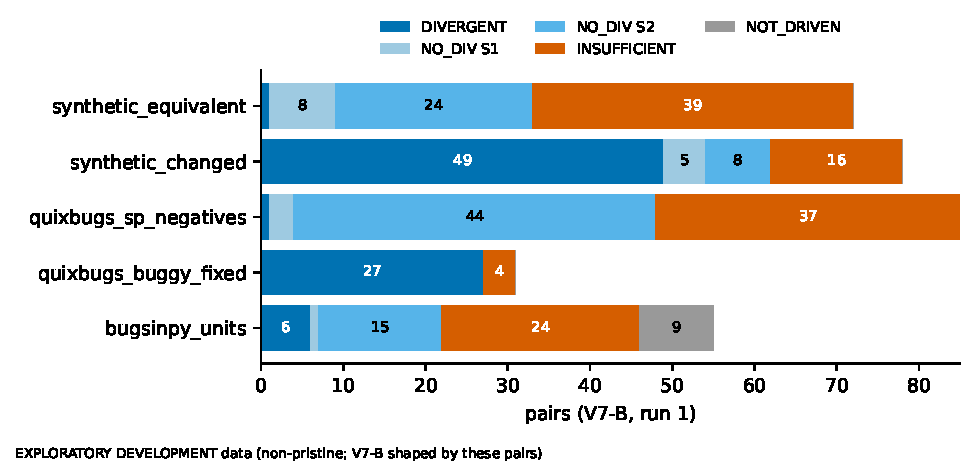
\includegraphics[width=\columnwidth]{../../results/postfix/figures/fig_verdict_sufficiency_by_dataset.pdf}
\caption{V7-B verdict and sufficiency per dataset (post-fix; source \path{results/postfix/figures/}, generated by \texttt{scripts/generate\_figures.py}). The earlier pre-fix versions are in \path{results/figures/} and are superseded.}\label{fig:verdictds}
\end{figure}
Table~\ref{tab:byarm} gives the verdict distribution per arm.
\begin{table}[t]
\centering\scriptsize
\caption{V7-B verdict and level per arm, all pairs including suspect and unlabelled (post-fix). Source: \path{paper/IEEE_ACCESS_INITIAL_MANUSCRIPT/tables/derived_crosstab.csv}.}
\label{tab:byarm}
\begin{tabular}{lrrrrr}
\hline
Arm & DIVERGENT & S2 & S1 & INSUFF. & Not driven \\
\hline
quixbugs\_buggy\_fixed & 27 & 0 & 0 & 4 & 0 \\
quixbugs\_sp\_negatives & 1 & 44 & 3 & 37 & 0 \\
synthetic\_changed & 49 & 8 & 5 & 16 & 0 \\
synthetic\_equivalent & 1 & 24 & 8 & 39 & 0 \\
bugsinpy\_units & 6 & 15 & 1 & 24 & 9 \\
\hline
\end{tabular}
\end{table}


\textbf{Paired comparison.} Table~\ref{tab:paired} compares against B1. V7-B has a lower false-assurance rate (improvement 0.104) but this is mostly outcomes relocating to \INS: V7-B abstains on 18 divergent-labelled pairs, and the lower detection (difference $-0.066$, 7 pairs in which only B1 succeeds, none the other way) is not significant after Holm correction. No row satisfies the +10pp rule. Matched-coverage false assurance (gate K4) was not computed, so these rows do not support any superiority claim. B3 detects four more pairs than B1 by mutation, a difference that is not significant.
\begin{table*}[t]
\centering\scriptsize
\caption{Paired comparisons against B1 (improvement is positive when better; b = test-only, c = reference-only successes). Unadjusted exploratory; no row meets the +10pp rule. Source: \path{results/postfix/statistics/paired_comparisons.csv}.}
\label{tab:paired}
\begin{tabular}{lrrrrrrrr}
\hline
Test & Outcome & Improv. & 95\% CI & b & c & p sign-flip & p Holm & +10pp \\
\hline
B1+rep & false assurance & -0.000 & [-0.000, -0.000] & 0 & 0 & 1.000 & 1.000 & False \\
B1+rep & detection & 0.000 & [0.000, 0.000] & 0 & 0 & 1.000 & 1.000 & False \\
B3 & false assurance & 0.038 & [0.007, 0.090] & 0 & 4 & 0.125 & 0.500 & False \\
B3 & detection & 0.038 & [0.007, 0.090] & 4 & 0 & 0.125 & 0.500 & False \\
V7-B & false assurance & 0.104 & [0.043, 0.205] & 0 & 11 & 0.001 & 0.006 & False \\
V7-B & detection & -0.066 & [-0.115, -0.026] & 0 & 7 & 0.031 & 0.156 & False \\
\hline
\end{tabular}
\end{table*}


\textbf{Negative finding 1: replay adds nothing measurable (B1+rep $\approx$ B1).} B1+rep equals B1 on all primary outcomes (zero discordant pairs in Table~\ref{tab:paired}). Over all 321 pairs the two differ on exactly 2 (B1 \DIV, B1+rep \texttt{NO\_DIFF}), both nondeterminism cases that V7-B reports as \INS{} (nondeterministic): a synthetic pair with a suspect label and a BugsInPy unit. The machinery of $r_{replay}=5$ and $k_{alt}=3$ shows no measurable value over repetition on these data, and the independent reviewer saw no witness demoted to environment-sensitive. V7-B costs roughly three times B1's CPU (Table~\ref{tab:metrics}).

\textbf{Negative finding 2: sufficiency does not visibly separate labels.} On synthetic pairs where B1 saw no difference, if sufficiency carried signal, S2 should be markedly purer in no-difference labels than \INS. Table~\ref{tab:suffsep} shows the shares are close (S2 holds 8 changed and 24 equivalent; \INS{} holds 11 and 23) and the direction for S1 is wrong. Labels are noisy and counts small, so this is not proof either way, but it is the only data and it is not supportive. Further, 16 of the 46 driven BugsInPy units, which are real fixes, received \NDO{} (15 at S2) on a synthetic battery, and 13 of 78 changed-labelled synthetic pairs received \NDO{}; S2 does not stop this failure mode.
\begin{table}[t]
\centering\scriptsize
\caption{V7-B outcome on synthetic pairs where B1 saw no difference, by generator label (suspect labels included, as in the red-team analysis). If sufficiency separated labels, S2 would be purer in EQUIVALENT than INSUFFICIENT; it is not clearly so. Source: \path{paper/IEEE_ACCESS_INITIAL_MANUSCRIPT/tables/derived_crosstab.csv}.}
\label{tab:suffsep}
\begin{tabular}{lrrr}
\hline
Generator label & V7-B S2 & V7-B S1 & V7-B INSUFFICIENT \\
\hline
CHANGED & 8 & 5 & 11 \\
EQUIVALENT & 24 & 8 & 23 \\
\hline
\end{tabular}
\end{table}


\textbf{Risk--coverage.} Table~\ref{tab:riskcov} and Fig.~\ref{fig:riskcov} show V7-B deciding fewer pairs (coverage 0.640 at all levels) with lower risk (0.079) than baselines that decide every pair (risk 0.271 for B1). Restricting to S2 lowers coverage and risk slightly. Risk is against generator labels with known defects, baselines have no sufficiency level, and this is a descriptive curve, not matched-coverage superiority.
\begin{table}[t]
\centering\scriptsize
\caption{Risk--coverage against generator labels. Baselines carry no sufficiency level, so their S-level rows are not comparable; V7-B at S3 is empty because S3 is never emitted. Source: \path{results/postfix/statistics/risk_coverage.csv}.}
\label{tab:riskcov}
\begin{tabular}{lrrrrr}
\hline
System & Min. level & Coverage & Risk & Decided & Eligible \\
\hline
B1 & none & 1.000 & 0.271 & 258 & 258 \\
B1 & S2 & 0.496 & 0.359 & 128 & 258 \\
B1 & S3 & 0.496 & 0.359 & 128 & 258 \\
B1+rep & none & 1.000 & 0.271 & 258 & 258 \\
B1+rep & S2 & 0.496 & 0.359 & 128 & 258 \\
B1+rep & S3 & 0.496 & 0.359 & 128 & 258 \\
B3 & none & 1.000 & 0.260 & 258 & 258 \\
B3 & S2 & 0.516 & 0.353 & 133 & 258 \\
B3 & S3 & 0.516 & 0.353 & 133 & 258 \\
V7-B & none & 0.640 & 0.079 & 165 & 258 \\
V7-B & S2 & 0.578 & 0.054 & 149 & 258 \\
V7-B & S3 & 0.291 & 0.000 & 75 & 258 \\
\hline
\end{tabular}
\end{table}

\begin{figure}[t]\centering
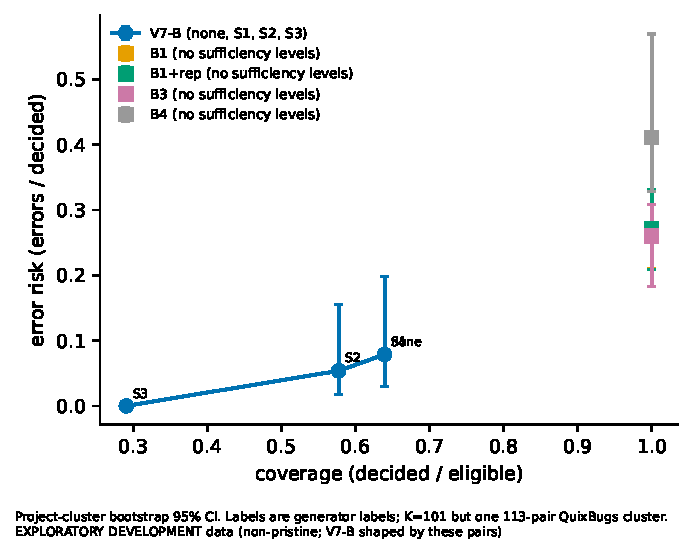
\includegraphics[width=\columnwidth]{../../results/postfix/figures/fig_risk_coverage.pdf}
\caption{Coverage versus error risk (post-fix; descriptive; generator labels; source \path{results/postfix/figures/}).}\label{fig:riskcov}
\end{figure}

\textbf{QuixBugs.} V7-B detected 27 of the 29 test-witnessed pairs (4 \INS: two loop forever in the buggy version, two are generator functions); B1, B1+rep and B3 detected 29 of 29; the edit-size heuristic B4 detected 1. There is no cluster interval because QuixBugs is one cluster (Fig.~\ref{fig:quix}).
\begin{figure}[t]\centering
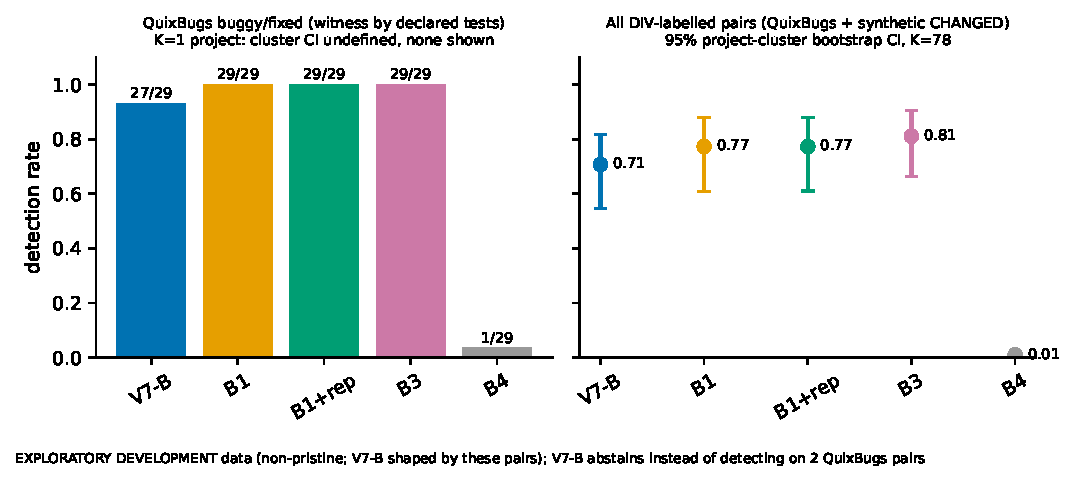
\includegraphics[width=\columnwidth]{../../results/postfix/figures/fig_detection_quixbugs_vs_baselines.pdf}
\caption{Detection on QuixBugs (one cluster) and on all divergent-labelled pairs with cluster intervals (source \path{results/postfix/figures/}); no superiority claim.}\label{fig:quix}
\end{figure}

\textbf{Class counts and runtime.} Table~\ref{tab:classcounts} lists verdict counts by truth class for V7-B and B1. Fig.~\ref{fig:runtime} shows CPU per pair; V7-B CPU is child-process time only and is a lower bound; memory was not recorded.
\begin{table}[t]
\centering\scriptsize
\caption{Verdict counts by truth class for V7-B and B1 (post-fix). Source: \path{results/postfix/statistics/class_counts.csv}.}
\label{tab:classcounts}
\begin{tabular}{lrrr}
\hline
System & Truth & Verdict & n \\
\hline
B1 & DIV & DIVERGENT\_OBSERVABLE & 82 \\
B1 & DIV & NO\_DIVERGENCE\_OBSERVED & 24 \\
B1 & NO\_OBS\_DIFF & DIVERGENT\_OBSERVABLE & 46 \\
B1 & NO\_OBS\_DIFF & NO\_DIVERGENCE\_OBSERVED & 106 \\
V7-B & DIV & DIVERGENT\_OBSERVABLE & 75 \\
V7-B & DIV & INSUFFICIENT & 18 \\
V7-B & DIV & NO\_DIVERGENCE\_OBSERVED & 13 \\
V7-B & NO\_OBS\_DIFF & INSUFFICIENT & 75 \\
V7-B & NO\_OBS\_DIFF & NO\_DIVERGENCE\_OBSERVED & 77 \\
\hline
\end{tabular}
\end{table}

\begin{figure}[t]\centering
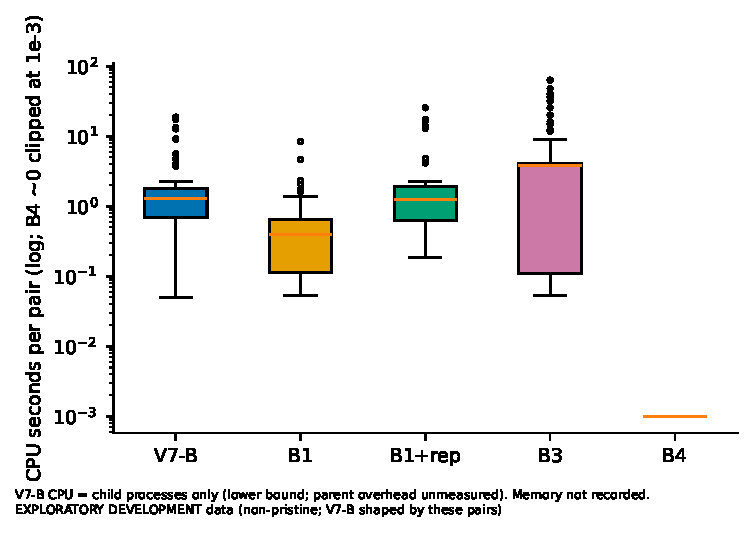
\includegraphics[width=\columnwidth]{../../results/postfix/figures/fig_runtime.pdf}
\caption{CPU seconds per pair per system, log scale (post-fix; V7-B child CPU only).}\label{fig:runtime}
\end{figure}

\textbf{Power.} Table~\ref{tab:power} shows that on the observed design (78 clusters, 106 pairs, discordance 0.066) power at +5pp is at most 0.27, and +10pp is not reachable because the observed discordance cannot carry a 10pp difference. This design cannot support a confirmatory claim.
\begin{table}[t]
\centering\scriptsize
\caption{Simulated power on the observed development design (K=78, 106 pairs, discordance 0.066); simulation assumptions A1--A4 are in the source file; not a prediction of system performance. Source: \path{results/postfix/statistics/power_actual.json}.}
\label{tab:power}
\begin{tabular}{lrrr}
\hline
ICC rho & alpha & Power +5pp & Power +10pp \\
\hline
0.0 & 0.05 & 0.267 & not reachable \\
0.0 & 0.0167 & 0.123 & not reachable \\
0.05 & 0.05 & 0.247 & not reachable \\
0.05 & 0.0167 & 0.095 & not reachable \\
0.15 & 0.05 & 0.215 & not reachable \\
0.15 & 0.0167 & 0.085 & not reachable \\
0.3 & 0.05 & 0.227 & not reachable \\
0.3 & 0.0167 & 0.068 & not reachable \\
\hline
\end{tabular}
\end{table}


\textbf{Determinism and crashes.} Whole-pair re-runs gave identical verdicts, levels, reasons and witness ids on every re-run pair (Table~\ref{tab:k1}); all 321 invocations produced a verdict with no engine crash. This shows the harness is stable on development pairs, not that verdicts are correct.
\begin{table}[t]
\centering\scriptsize
\caption{K1 spike per-arm counts and whole-pair re-run determinism (post-fix; the synthetic arm was not re-run after the fix). K1 itself is NOT MET. Source: \path{results/postfix/processed/k1_spike_summary.json}.}
\label{tab:k1}
\begin{tabular}{lrrrrr}
\hline
Arm & Pairs & Runnable & Projects & Re-run & Identical \\
\hline
quixbugs & 31 & 30 & 1 & 31 & 31 \\
quixbugs\_neg & 85 & 54 & 1 & 25 & 25 \\
synthetic & 150 & 132 & 101 & 0 & 0 \\
bugsinpy\_units & 55 & 44 & 12 & 46 & 46 \\
\hline
\end{tabular}
\end{table}


\section{Ablation, Sensitivity, Generalisation and Runtime}\label{sec:ablation}
\textbf{Ablation: \NE.} No component ablation of V7-B was run (replay, control alternation, sufficiency floors, exploration). The only proxy is B1 versus B1+rep, which isolates the repetition machinery from sufficiency (Section~\ref{sec:results}); it cannot isolate the sufficiency gate, because B1+rep also lacks it. Result files from earlier-generation systems exist in the repository (\path{results/ablations/} and the \texttt{results/phase*} directories) and are not V7-B results and are not used here.

\textbf{Sensitivity: \NE{} for thresholds and budgets.} The 0.80 branch floor, repeat counts and the CPU-budget grid were not varied. The one sensitivity analysis performed excludes renamed-entry pairs (Section~\ref{sec:results}).

\textbf{Generalisation: \NE.} Nothing supports generalisation across projects, domains, languages or platforms (Section~\ref{sec:limitations}); there is no independent real-project run.

\textbf{Runtime: lower bound only.} V7-B's median CPU per pair is about 1.3~s (child processes only; parent overhead unmeasured; memory not recorded; one machine, four workers, at most 12 inputs per pair). See Fig.~\ref{fig:runtime} and Table~\ref{tab:metrics}.

\section{Failure Analysis}\label{sec:failure}
This section describes observed failure modes in the development data (Table~\ref{tab:reasons}).
\begin{itemize}
\item \textbf{Engine coverage gaps dominate \INS.} Of 120 \INS{} primary reasons overall, 60 are \texttt{changed\_region\_not\_activated} (the inputs never reached the changed lines, expected for batteries not written for the bug) and 49 are \texttt{unsupported\_signature} from renamed entries, which the engine cannot handle. Generator functions are not consumed, so their bodies never run (QuixBugs flatten and kheapsort). Eight BugsInPy class units are not driven. The \INS{} rate is therefore not evidence of honest abstention.
\item \textbf{Resource limits.} After the fix there are 7 \texttt{resource\_limit} outcomes; three quixbugs negatives moved from \NDO{} to \INS{} when the no-run defect was fixed. An infinite loop introduced in one version is reported as its own stratum, not a witness.
\item \textbf{\NDO{} on pairs known to differ.} 16 of 46 driven real-fix units and 13 of 78 changed-labelled synthetic pairs received \NDO, i.e.\ the battery did not reach the differing behaviour; S2 does not prevent this.
\item \textbf{Label strictness.} The boundary treats the type tag as identity, so a semantics-preserving rewrite returning a boolean for an integer yields a witness (two labelled-equivalent pairs, not adjudicated); six suspect labels are excluded from denominators.
\item \textbf{Capture gaps.} Output written through the file descriptor directly, or by subprocesses, bypasses capture; control alternation virtualises only seeded random and the clock, not other entropy sources, so environment-sensitivity detection is partial.
\item \textbf{Defect.} The reachability of \NDO{} with a no-run input (Section~\ref{sec:verdicts}), found by the independent review, was fixed; three pairs changed.
\end{itemize}
\begin{table}[t]
\centering\scriptsize
\caption{Primary reasons for INSUFFICIENT per arm (post-fix). Most are engine coverage gaps (renamed entries, generators, class units), not a sufficiency judgement. Source: \path{results/postfix/processed/k1_spike_summary.json}.}
\label{tab:reasons}
\begin{tabular}{lrr}
\hline
Arm & Primary INSUFFICIENT reason & n \\
\hline
quixbugs & resource\_limit & 2 \\
quixbugs & changed\_region\_not\_activated & 2 \\
quixbugs\_neg & unsupported\_signature & 31 \\
quixbugs\_neg & changed\_region\_not\_activated & 3 \\
quixbugs\_neg & resource\_limit & 3 \\
synthetic & changed\_region\_not\_activated & 34 \\
synthetic & unsupported\_signature & 18 \\
synthetic & resource\_limit & 2 \\
synthetic & nondeterministic & 1 \\
bugsinpy\_units & changed\_region\_not\_activated & 21 \\
bugsinpy\_units & nondeterministic & 1 \\
bugsinpy\_units & import\_error & 1 \\
bugsinpy\_units & unobservable\_outcome & 1 \\
bugsinpy\_units & class unit & 8 \\
\hline
\end{tabular}
\end{table}


\section{Discussion}\label{sec:discussion}
The implementation shows that a closed, traceable three-verdict contract is feasible for Python functions. The data, however, do not show that the distinguishing element, the sufficiency level, adds value. Plain repetition reproduces V7-B's flakiness handling at similar protection; V7-B's lower false assurance is largely relocation to \INS{}, and \INS{} is itself dominated by features the engine does not implement. Where V7-B differs from B1 most visibly (renamed entries) the difference is a refusal rather than a finding. An independent review's readiness verdict was that the work is publishable only as a design, feasibility or negative-result report, with the honest alternative that the contribution is better framed as an evidence contract for differential testing than as a sufficiency advance. We adopt that framing.

What a decisive study would need: independent labelled real pairs with a kappa-checked truth team; a sealed holdout; matched-coverage false-assurance comparison of V7-B against B1+rep; at least one published tool (Testora, DiffTestGen or Mokav class) or dropping competitive claims; and engine support for renames, generators and class units so that \INS{} carries meaning. Current data predict, but do not establish, that sufficiency would show little gain over B1+rep.

\section{Threats to Validity}\label{sec:threats}
\textbf{Internal.} V7-B was tuned and debugged on the evaluated pairs; the baselines B4 and B5 were fitted on development material; synthetic labels are generator labels, not adjudicated, and at least two are wrong under V7-B's boundary; the BugsInPy units have no truth label; the S1/S2 thresholds are unvalidated defaults; the sufficiency level is a coverage proxy with a known weak link to fault detection~\cite{inozemtseva2014coverage,just2014mut}; one constant-true channel check and the ignorance of input count weaken S2. Label noise and duplication are known to distort evaluations~\cite{allamanis2019,jimenez2019}.
\textbf{Construct.} ``False assurance'' is measured against labels that may not be true divergences; ``abstention'' is dominated by unimplemented features; CPU is child-only.
\textbf{External.} Python top-level functions with JSON arguments; one machine; macOS \texttt{sandbox-exec}; CPython 3.13 only; QuixBugs counts as a single cluster; synthetic projects are generator programs; the effective number of independent projects is not assessable. Leakage and non-independence are expected~\cite{kapoor2023leakage}.
\textbf{Statistical.} Percentile bootstrap intervals undercover with a small effective number of clusters and one dominant cluster; the estimated intraclass correlation of zero is unreliable; power is low (Table~\ref{tab:power}); randomisation-related guidance for evaluations~\cite{arcuri2012a,klees2018evaluating} is only partly applicable. Comparisons are unadjusted exploratory; no multiplicity claim is made.
\textbf{Review.} The literature review is single-reviewer, abstract-level for most sources; absence claims are not proofs.

\section{Limitations}\label{sec:limitations}
Not implemented: S3; the explorer and input generation (inputs are user JSON values only); module E; entry lifting and declared renames; generator and class entries; Merkle commitments, supersession, minimisation and event-stream storage; interpreter-mismatch handling; Linux and container isolation. Four specified reason codes are never emitted. The branch-coverage metric is conservative and the all-channels-instrumented check is constant. Isolation on macOS is below the specification's own minimum; reads are unconfined. Control alternation covers only seeded random and the clock. Quarantine is conservative; stopping at budget with unrun inputs but all changed units hit can still yield \NDO{}; an empty changed region yields a vacuous activation that can still reach \NDO. All evaluation data are non-pristine; K1 is not met; no confirmatory evaluation, no independent ground truth and no sealed holdout exist; the study is under-powered; no published tool was compared; no overhead beyond a lower bound is available. Results on the earlier-generation systems must not be conflated with V7-B.

\section{Conclusion}\label{sec:conclusion}
We described V7-B, a witness-based differential comparison with a closed three-verdict contract and a recorded sufficiency level, implemented for Python functions with S0--S2 and without S3. On 321 exposed development pairs the implementation is deterministic and crash-free, but the exploratory data show a null replay effect over plain repetition, no visible separation of labels by sufficiency, lower detection than same-input differential execution, and abstention driven by engine gaps. The feasibility gate K1 is not met, the design is under-powered, and no published tool was compared. The work stands as a design, feasibility and negative-result report; a confirmatory study with independent labelled real pairs and a matched-coverage comparison against repetition-based baselines is required before any claim of benefit.

\bibliographystyle{IEEEtran}
\bibliography{references}
\end{document}
